\documentclass[12pt,a4paper,fleqn]{article}
\title{Progress Report}
\author{Syed Ahmad Raza}
\date{2018.05.02}
\usepackage{mathtools}
\usepackage{graphicx}
\usepackage{color}          % for color eps output
%\usepackage{afterpage}
\usepackage{float}          % to force a figure placement with [H] command
\usepackage{enumitem}
\usepackage{newtxtext}
\usepackage{newtxmath}
\usepackage{nicefrac}
%\usepackage{layouts}       % for: \printinunitsof{in}\prntlen{\textwidth}

\begin{document}
\maketitle
%\tableofcontents
%\pagebreak

\section{2D FVD solver Navier-Stokes using two layers of ghost cells}

\subsection{Ghost cells}
Two layers of ghost cells were implemented in C++ using Finite Volume Method to solve the Navier-Stokes equations, as shown in the following figure for a reduced grid size.

\begin{figure}[H]
    \centering
    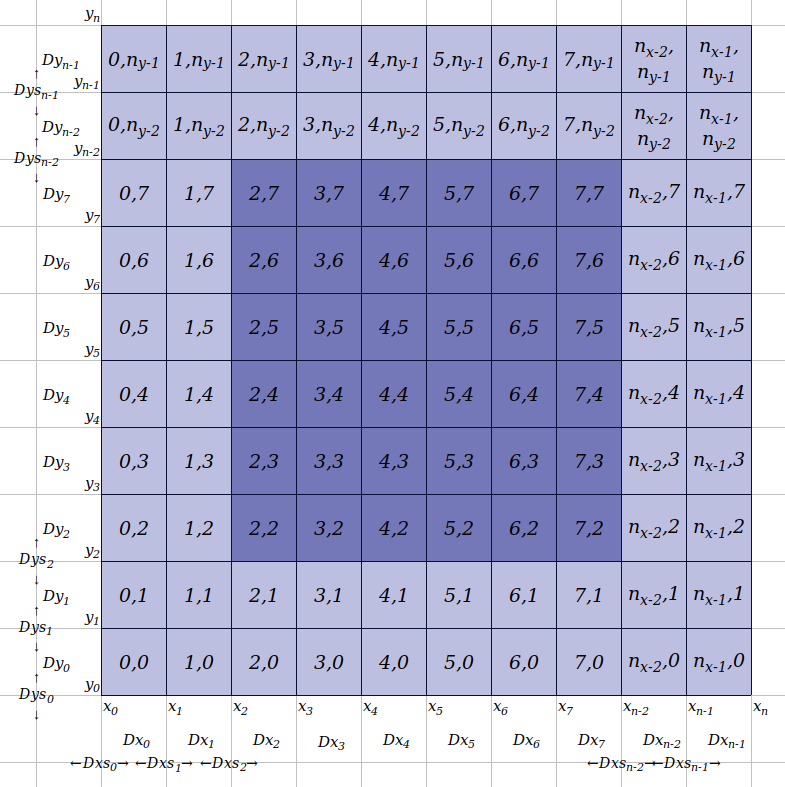
\includegraphics[width=0.65\linewidth]{../figures/grid_overview.png}
    \caption{Figure representing the utilization of two ghost cells around the grid, for grid of reduced size}
\end{figure}

\subsection{Debugging}
Earlier code had a major bug, which  in that it implemented the far-side velocity boundary conditions incorrectly. The corrected velocity boundary conditions in the x and y directions for the far side are given below.

\(u\)-velocity for the east boundary:
\begin{equation}
u_{n_x-3,j} = 0\\
u_{n_x-2,j} = u_{n_x-3,j}
\end{equation}

\(v\)-velocity for the north boundary:
\begin{equation}
v_{i,n_y-3} = 0\\
v_{i,n_y-2} = v_{i,n_y-3}
\end{equation}

This can be understood with the help of the following figure.

\begin{figure}[H]
    \centering
    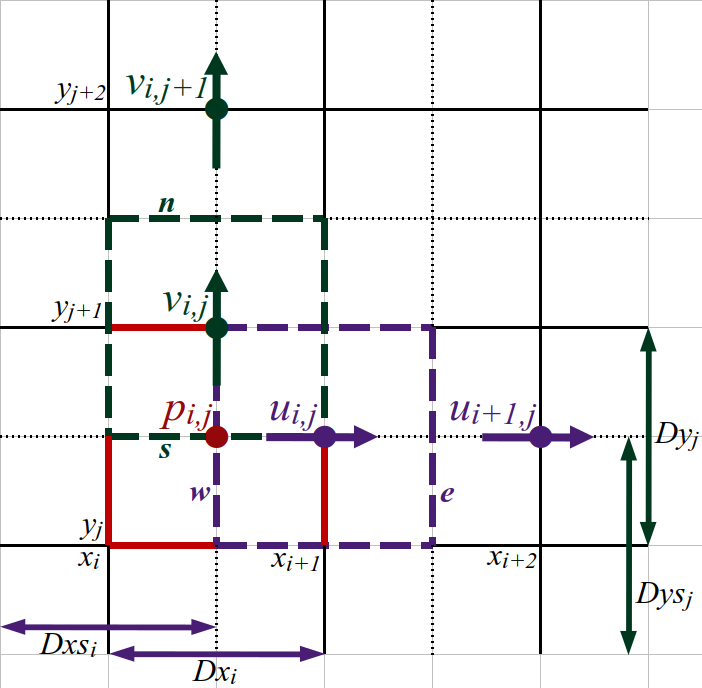
\includegraphics[width=0.9\linewidth]{../figures/grid_staggered.png}
    \caption{Representation of the utilization of two ghost cells around the grid, for grid of reduced size}
\end{figure}

\subsection{Results}
The code was solved for the case of a lid-driven cavity flow in a two-dimensional square box. The results are shown in the following figures.

\begin{figure}[H]
    \centering
    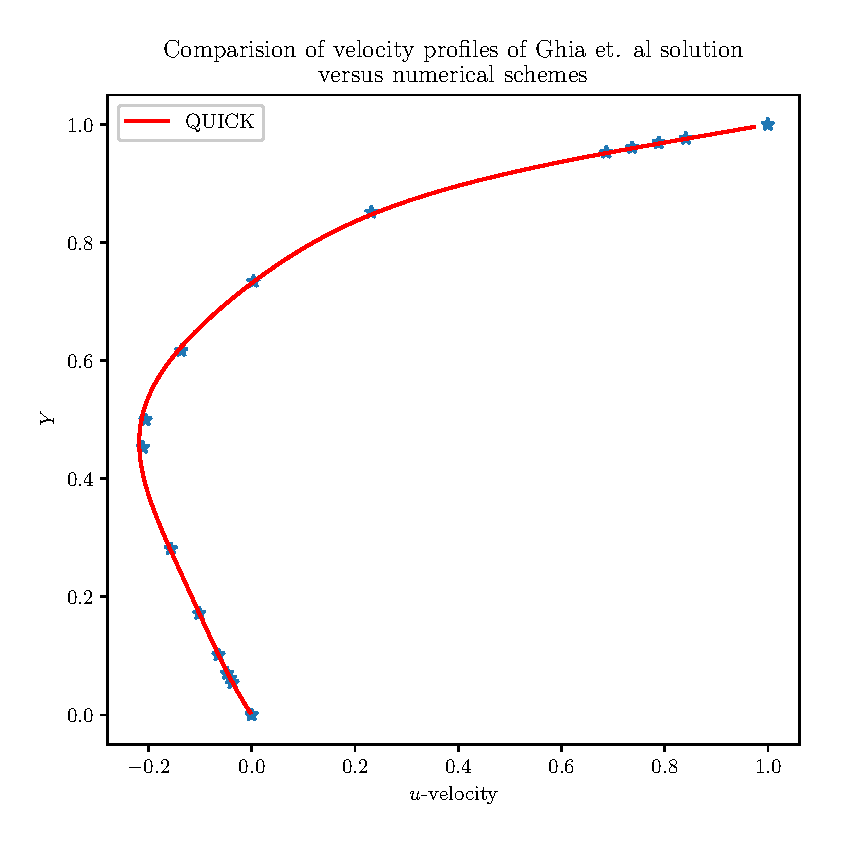
\includegraphics[width=\linewidth]{n,xy=121_050213_qk_cavityFlowU.eps}
    \caption{Comparing the solution provided by Ghia et. al versus the numerical solution for \(u\)-velocity values for all \(y\) at the center of \(x\) -axis, for a 121\(\times\)121 grid.}
\end{figure}

\begin{figure}[H]
    \centering
    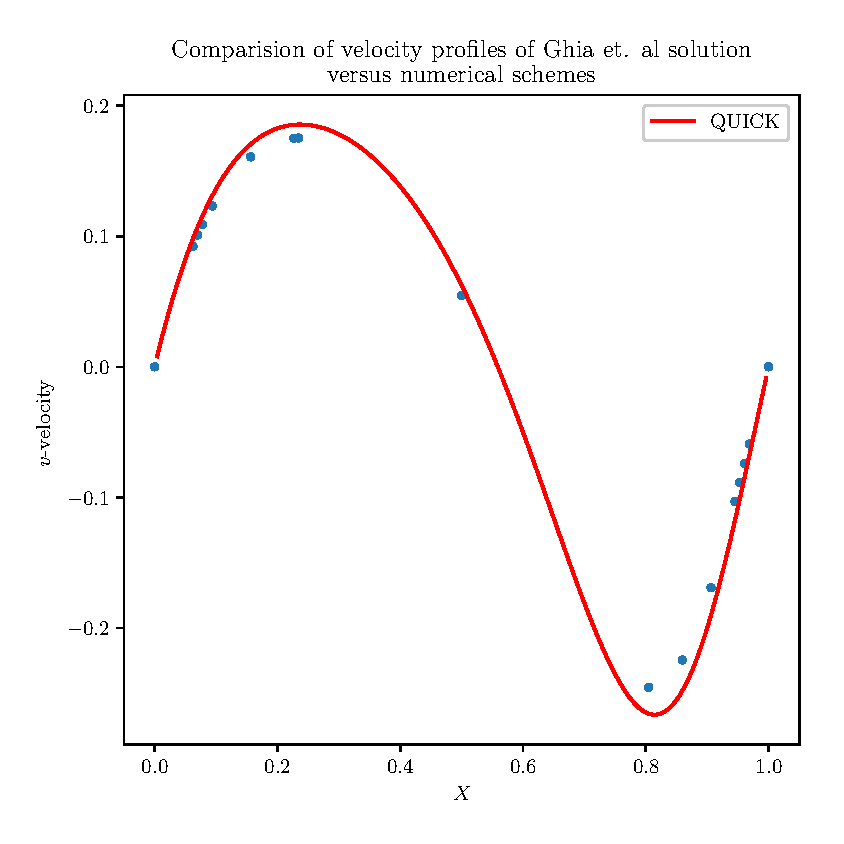
\includegraphics[width=\linewidth]{n,xy=121_050213_qk_cavityFlowV.eps}
    \caption{Comparing the solution provided by Ghia et. al versus the numerical solution for \(v\)-velocity values for all \(x\) at the center of \(x\) -axis, for a 121\(\times\)121 grid.}
\end{figure}

\subsection{Ongoing tasks}
\begin{enumerate}
    \item Calculating the virtual force for a cylinder inside a lid-driven cavity
    \item Employ parallel computing by using ultraMPP C++ library to execute the code on parallel cores
    \item Solve cavity-driven flow for 3D
\end{enumerate}

\end{document}
